
\begin{figure}
\center

	\begin{subfigure}[t]{0.22\textwidth}
		\center
		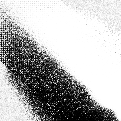
\includegraphics[width=\stratgraphwidth]{images/findings/experiments/neighbors/strats/hand_max_min.png}
		\caption{\handmaxmin}
	\end{subfigure}
	~
	\begin{subfigure}[t]{0.22\textwidth}
		\center
		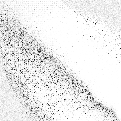
\includegraphics[width=\stratgraphwidth]{images/findings/experiments/neighbors/strats/hand_max_avg.png}
		\caption{\handmaxavg}
	\end{subfigure}
~
	\begin{subfigure}[t]{0.22\textwidth}
		\center
		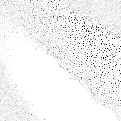
\includegraphics[width=\stratgraphwidth]{images/findings/experiments/neighbors/strats/hand_max_med.png}
		\caption{\handmaxmed}
	\end{subfigure}
	~
	\begin{subfigure}[t]{0.22\textwidth}
		\center
		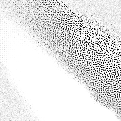
\includegraphics[width=\stratgraphwidth]{images/findings/experiments/neighbors/strats/hand_max_poss.png}
		\caption{\handmaxposs}
	\end{subfigure}

	\begin{subfigure}[t]{0.22\textwidth}
		\center
		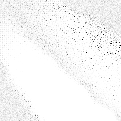
\includegraphics[width=\stratgraphwidth]{images/findings/experiments/neighbors/strats/crib_min_avg.png}
		\caption{\cribminavg}
	\end{subfigure}
	~
	\begin{subfigure}[t]{0.22\textwidth}
		\center
		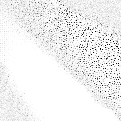
\includegraphics[width=\stratgraphwidth]{images/findings/experiments/neighbors/strats/pegging_max_avg_gained.png}
		\caption{\peggingmaxavggained}
	\end{subfigure}
~
	\begin{subfigure}[t]{0.22\textwidth}
		\center
		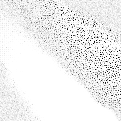
\includegraphics[width=\stratgraphwidth]{images/findings/experiments/neighbors/strats/pegging_max_med_gained.png}
		\caption{\peggingmaxmedgained}
	\end{subfigure}
	~
	\begin{subfigure}[t]{0.22\textwidth}
		\center
		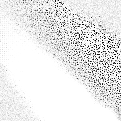
\includegraphics[width=\stratgraphwidth]{images/findings/experiments/neighbors/strats/pegging_min_avg_given.png}
		\caption{\peggingminavggiven}
	\end{subfigure}

\caption{
	Final strategy graphs for an agent when playing as the pone
	after being trained for 500,000 games
	by following a policy which uses a weighted sum of neighboring weights.
}
\label{fig:neighbor-strats}
\end{figure}
